\chapter{Introdução}
\label{cap:introducao}
Considerado como ponto chave para a Web Semântica \cite{berners2001semantic}, Dados Conectados vem sendo abordado de forma crescente por acadêmicos, governos e empresas. Tal crescimento se deve ao fato de Dados Conectados ser uma alternativa relevante para conectar bases de dados distribuídas na Web. Segundo \citeonline{hyland2011joy}, Dados Conectados se trata de um conjunto de boas práticas para publicar e conectar dados estruturados na Web. Ademais, \citeonline{berners2006linked} afirma que não se trata apenas de por dados na internet, mas fazer conexões entre eles, permitindo assim, que pessoas ou máquinas possam explorar a Web dos dados.

Web de Dados bem como Web dos Documentos, são termos utilizados para descrever o paradigma da Web atualmente, onde o primeiro, que tem como base o segundo, reflete a possibilidade de conectar os dados através de links. Sendo esta, uma possibilidade inexistente quando se fala de Web dos Documentos, pois nesta, os documentos apontam para outros documentos através de links.

Dados Conectados pode ser visto sob duas perspectivas: consumo e publicação. A primeira aborda o ponto de vista do consumidor, tratando a exploração de dados para tornar as aplicações mais ricas. A segunda está sob a perspectiva do publicador, abordando processos \cite{bizer2007publish, hyland2011joy, villazon2011methodological, Avila2015} e conceitos \cite{berners2006linked, wood2014linked} necessários para publicar e manter os dados na Web de forma conectada. 

Publicar ou manter dados conectados na Web vai além de disponibilizar conjuntos de dados através de serializações RDF. É necessário conectá-los a outros conjuntos de dados já existentes. Porém, criar links entre conjuntos de dados requer uma análise cuidadosa por parte do especialista, que apesar de ser uma abordagem eficaz, não é escalável, visto que a quantidade de dados publicados cresce constantemente. Consequentemente, inviabilizando o processo de publicação de forma artesanal. Logo, para que seja possível constuir a Web de Dados de forma eficiente, é necessário que existam soluções capazes de conectar dados de forma automática ou semi-automática.

Conectar dados automaticamente é um problema reconhecido por diversas comunidades. Dentre essas comunidades, podemos destacar as comunidades de Bancos de Dados e Web Semântica. Na primeira, esse problema é conhecido através do termo \textbf{\textit{Record Linkage}} \cite{gu2003record}. Na segunda, ele é reconhecido pelo termo \textbf{\textit{Instance Matching}}. Além disso, também é possível encontrar referências como \textbf{\textit{Problema de Resolução de Entidades}} \cite{menestrina2005generic} e \textbf{\textit{Deduplicação}} \cite{sarawagi2002interactive}, que se trata de um processo que tem como objetivo identificar e mesclar recursos julgados representar a mesma entidade do mundo real.
%\begin{itemize}
%    \item \textbf{Integração semântica de dados}: Refere-se ao melhoramento de as técnicas existentes pra descobertas de mapeamento (semi) automático entre ontologias heterogêneas e distribuídas; 

%    \item \textbf{Reconhecimento de identidade}: Refere-se à capacidade de identificar se descritores de recursos distintos estão relacionados à mesma entidade do mundo real; 

%    \item \textbf{População de ontologias}: Refere-se a descoberta de relacionamentos entre novas instâncias e as instâncias já existentes na base de conhecimento. 
%\end{itemize}

%Por exemplo, admitindo a existência de uma entidade do mundo real (e.g. Pesquisador) onde atributos como nome e endereço estão armazenados em datasets distintos, onde estão vinculados a recursos que usam as seguintes URIs (http://www.ic.ufal.br/dac/rbie/author/615 e http://lattes.cnpq.br/4038730280834132) como na Figura \ref{fig:modelo_semantico}. Neste cenário, não é possível determinar, apenas através do alinhamento entre as ontologias, que ambas URIs fazem referência a mesma entidade, sendo necessário analisar informações adicionais provenientes de conexões semânticas entre conceitos e relações presentes nestes dados [31, 35]. 

%\begin{figure}[!ht]
%	\centering
%	\includegraphics[width=0.95\textwidth]{./imagens/researcher.png}\\
%    \caption{Relação entre entidade do mundo real, dados e modelo semântico}
%	\footnotesize{Fonte: Próprio autor.}
%	\label{fig:modelo_semantico}
%\end{figure}
%No cenário de publicação de Dados Conectados, criar conexões entre conjuntos de dados é uma tarefa custosa, pois requer análise preliminar e detalhada por um especialista de domínio. 

%Além disso, com a crescente quantidade de dados que estão sendo publicados Web, conforme a Figura \ref{fig:oferta_2020}, conectar esses dados se torna cada vez mais desafiador. Por exemplo, o catálogo de dados do governo de São Paulo2, que até o presente momento contém 424 conjuntos de dados, possui apenas 13 (0.23\%) que disponibiliza seus dados através de alguma serialização RDF (Turtle, RDF/XML).  


%AQUI, PRECISA ESCREVER SOBRE TÉCNICAS APLICADAS POR OUTROS TRABALHOS (RELACIONADOS) E DIZER POR QUE ELES NÃO RESOLVEM O PROBLEMA.  

%DEPOIS DISSO, DIZER QUE UM CAMINHO DE SOLUÇÃO É O ALINHAMENTO USANDO XXXXXXXXX E/OU YYYYYYYYYYY.  

%Dessa forma, pretende-se dispor uma abordagem semi-automática para publicar Dados Conectados, a partir de dados estruturados (publicado e não publicados na Web), levando em consideração, técnicas de alinhamento de dados, contribuindo assim, para o cenário de publicação de Dados Conectados. 

%Figura 2 - Oferta de dados na Web até 2020. Fonte: EMC 2012 
%\begin{figure}[!ht]
%	\centering
%	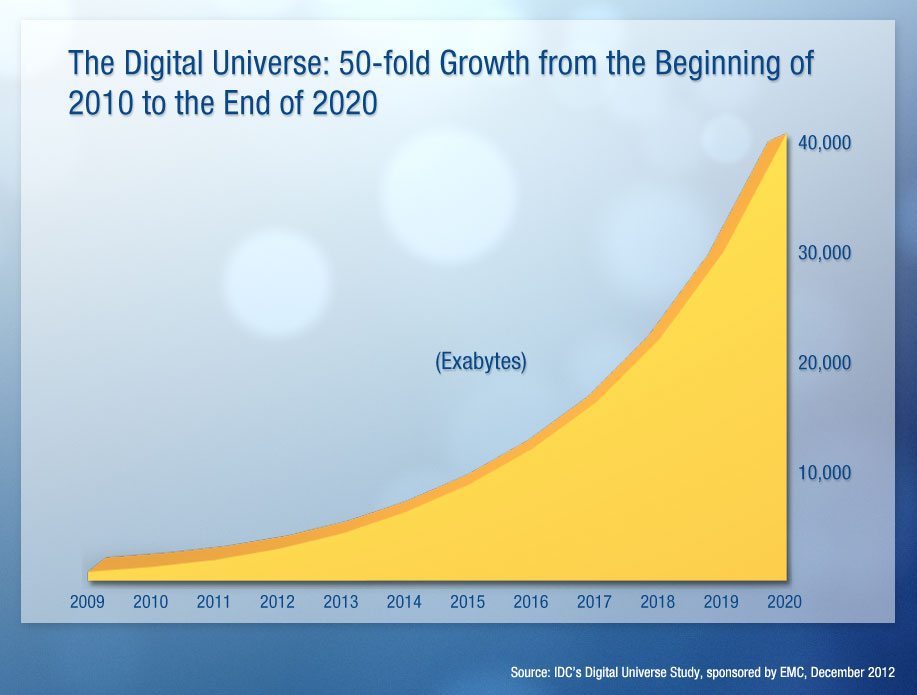
\includegraphics[width=0.8\textwidth]{./imagens/oferta.png}\\
%    \caption{Oferta de dados na Web até 2020}
%	\footnotesize{Fonte: EMC 2012.}
%	\label{fig:oferta_2020}
%\end{figure}



\subsection*{Contextualização}

\subsection*{Problemática}

\subsection*{Solucionática}

\subsection*{Objetivos}

\subsubsection*{Objetivo Geral}

\begin{itemize}
	\item Objetivo geral.
\end{itemize}

\subsubsection*{Objetivos específicos}
\begin{itemize}
\item Objetivo específico 1;
\item Objetivo específico 2;
\item Objetivo específico 3;
\item Objetivo específico 4.
\end{itemize}

\subsection*{Estrutura do trabalho}

O restante do trabalho está estruturado como segue:

\begin{enumerate}
\item[a)] \textbf{Seção 2} - descrição;
\item[b)] \textbf{Seção 3} - descrição;
\item[c)] \textbf{Seção 4} - descrição;
\item[d)] \textbf{Seção 5} - descrição;
\item[e)] \textbf{Seção 6} - descrição;
\item[f)] \textbf{Seção 7} - descrição;
\end{enumerate}
